\begin{figure}[ht]
\centering
% Thesis-wide categorical color palette
% Usage: % Thesis-wide categorical color palette
% Usage: % Thesis-wide categorical color palette
% Usage: \input{figures/palette} in any figure file
%
% Muted primary colors -- print-friendly, visually distinct.
% Inspired by Cooper Union's red/blue primaries, softened for
% academic figures. Use palA-palC for data series in scatter
% plots, line charts, bar charts, etc.

\definecolor{palA}{HTML}{1F77B4}   % Tableau blue
\definecolor{palB}{HTML}{D62728}   % Tableau red
\definecolor{palC}{HTML}{2CA02C}   % Tableau green
 in any figure file
%
% Muted primary colors -- print-friendly, visually distinct.
% Inspired by Cooper Union's red/blue primaries, softened for
% academic figures. Use palA-palC for data series in scatter
% plots, line charts, bar charts, etc.

\definecolor{palA}{HTML}{1F77B4}   % Tableau blue
\definecolor{palB}{HTML}{D62728}   % Tableau red
\definecolor{palC}{HTML}{2CA02C}   % Tableau green
 in any figure file
%
% Muted primary colors -- print-friendly, visually distinct.
% Inspired by Cooper Union's red/blue primaries, softened for
% academic figures. Use palA-palC for data series in scatter
% plots, line charts, bar charts, etc.

\definecolor{palA}{HTML}{1F77B4}   % Tableau blue
\definecolor{palB}{HTML}{D62728}   % Tableau red
\definecolor{palC}{HTML}{2CA02C}   % Tableau green

\definecolor{nodeblue}{HTML}{B8D2E6}
\definecolor{nodeborder}{HTML}{5A87B5}
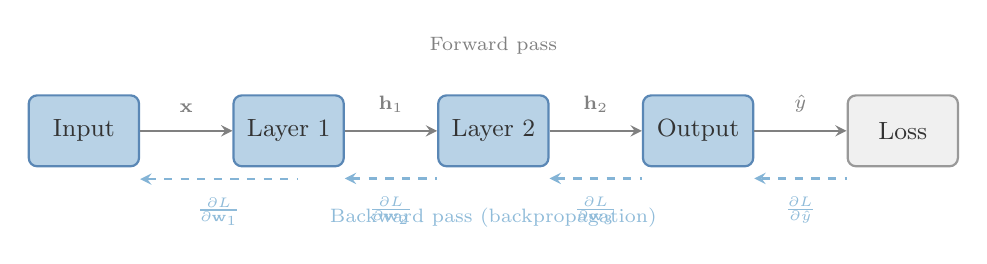
\begin{tikzpicture}[
    block/.style={draw=nodeborder, thick, fill=nodeblue,
                  rounded corners=3pt, minimum width=1.4cm,
                  minimum height=0.9cm, font=\small,
                  text=black!80},
    lossblock/.style={draw=black!40, thick, fill=black!6,
                      rounded corners=3pt, minimum width=1.4cm,
                      minimum height=0.9cm, font=\small,
                      text=black!80},
    fwd/.style={->, thick, >=stealth, black!50},
    bwd/.style={<-, thick, >=stealth, dashed, palA!55},
    lbl/.style={font=\scriptsize, text=black!50},
    bwdlbl/.style={font=\scriptsize, text=palA!50},
]

% --- Blocks ---
\node[block] (input) at (0, 0) {Input};
\node[block] (h1)    at (2.6, 0) {Layer 1};
\node[block] (h2)    at (5.2, 0) {Layer 2};
\node[block] (out)   at (7.8, 0) {Output};
\node[lossblock] (loss) at (10.4, 0) {Loss};

% --- Forward pass (solid arrows, above) ---
\draw[fwd] (input.east) -- (h1.west)
    node[midway, above=3pt, lbl] {$\mathbf{x}$};
\draw[fwd] (h1.east) -- (h2.west)
    node[midway, above=3pt, lbl] {$\mathbf{h}_1$};
\draw[fwd] (h2.east) -- (out.west)
    node[midway, above=3pt, lbl] {$\mathbf{h}_2$};
\draw[fwd] (out.east) -- (loss.west)
    node[midway, above=3pt, lbl] {$\hat{y}$};

% Forward label
\node[lbl, anchor=south] at (5.2, 0.85) {Forward pass};

% --- Backward pass (dashed arrows, below) ---
\draw[bwd] (input.south east) ++(0, -0.15)
    -- ++(2.0, 0)
    node[midway, below=3pt, bwdlbl]
    {$\frac{\partial L}{\partial \mathbf{w}_1}$};
\draw[bwd] ([yshift=-4pt]h1.south east)
    -- ([yshift=-4pt]h2.south west)
    node[midway, below=3pt, bwdlbl]
    {$\frac{\partial L}{\partial \mathbf{w}_2}$};
\draw[bwd] ([yshift=-4pt]h2.south east)
    -- ([yshift=-4pt]out.south west)
    node[midway, below=3pt, bwdlbl]
    {$\frac{\partial L}{\partial \mathbf{w}_3}$};
\draw[bwd] ([yshift=-4pt]out.south east)
    -- ([yshift=-4pt]loss.south west)
    node[midway, below=3pt, bwdlbl]
    {$\frac{\partial L}{\partial \hat{y}}$};

% Backward label
\node[bwdlbl, anchor=north] at (5.2, -0.85) {Backward pass
    (backpropagation)};

\end{tikzpicture}
\caption{Forward and backward passes through a neural network. Solid
  arrows (top): input flows left to right through each layer to
  produce a prediction and a loss. Dashed arrows (bottom): gradients
  flow right to left from the loss back through each layer, telling
  each weight how to change.}
\label{fig:forward-backward}
\end{figure}
